\section{E-Logbook}
E-Logbook adalah sebuah buku elektronik untuk mencatat catatan/dokumen penting secara detail setiap aktivitas yang berisi masalah-masalah yang membutuhkan tindak lanjut dari pihak yang terlibat dalam satu hari penuh. Seluruh pegawai sebaiknya membaca buku ini agar mengetahui kegiatan, kerusakan, dan target pekerjaan apa saja yang dilakukan hari sebelumnya. Ada beberapa manfaat e-logbook antara lain:
\begin{enumerate}
\item bahan bukti untuk merekap seluruh aktivitas
\item bahan pembuatan laporan kegiatan
\item alat untuk memudahkan pegawai dalam merekap kegiatan
 \end{enumerate}

Hal yang perlu di isi dalam e-logbook ini antara lain:
\begin{enumerate}
\item Hari, tanggal dan tahun
\item Nama pegawai yang dinas pada hari tersebut
\item Nama vendor yang dinas pada hari tersebut
\item Penerbangan hari ini
\item Kegiatan
\item Kerusakan
\item Target pekerjaan
\end{enumerate}


\subsection{Mengaktifkan MySQLi}
Kenapa disini kita membahas tentang cara mengaktifkan MySQLi karena PHP 5 keatas default-nya menggunakan platform MySQLi untuk menggunakan berbagai fungsi pada database MySQL. MySQLi adalah sebuah class di PHP, jadi pastikan bahwa versi PHP kita sudah 5 keatas yaa.
Keunggulan menggunakan MySQLi ketimbang dengan MySQL:
\begin{enumerate}
\item Dukungan baru untuk keperluan transaksi
\item Prosedur interface
\item Susunan laporan lebih tersusun
\item Debugging lebih ditingkatkan
\item Dapat memproses dalam waktu yang lebih singkat
\end{enumerate}

Nah itu beberapa keunggulan menggunakan MySQLi. Dan sekarang kita akan membahas cara mengaktifkan MySQLi pada PHP.
Untuk mengaktifkan MySQLi, langkah pertama update dahulu versi PHP kita ke PHP 5 keatas. kemudian cari file php.ini biasanya terdapat di folder C lalu folder xampp lalu folder php kemudian buka file php.ini menggunakan editor seperti notepad++, sublime text, dan adobe dreamweaver. Tambahkan skrip extension=php\_mysqli.dll pada file php.ini. Namun pada file php.ini sudah ada skrip extension=php\_mysqli.dll dan terdapat tanda ; (tanpa tanda kutip) di depanya, maka kita cukup menghapus tanda ; tersebut lalu simpan file php.ini yang sudah di edit. Jangan lupa untuk restart server apachenya.

\subsection{Langkah Pertama}
Agar dapat menjalankan sistem yang akan dibuat, kita harus menginstall aplikasi web server yang mendukung PHP ini serta aplikasi untuk database MySQL. Untungnya terdapat banyak aplikasi yang menghandle program ini, salah satunya yaitu XAMPP. Aplikasi XAMPP adalah aplikasi yang dapat menghandle banyak aplikasi lain yang dibutuhkan untuk pengembangan web. Nama XAMPP adalah singkatan dari X (huruf X berarti cross-platform), A (Apache web server), M (MySQL), P (PHP), dan P (Perl). Selain beberapa aplikasi tersebut XAMPP menyediakan modul lain seperti OpenSSL dan phpMyAdmin.
\par
Cara mendownload XAMPP terbaru bisa di situs resminya yaitu www.apachefriends.org. Untuk versi terbaru sudah support untuk PHP 7, silahkan pilih download sesuai dengan sistem operasi yang kita pakai.
\begin{figure}[h]
\centering
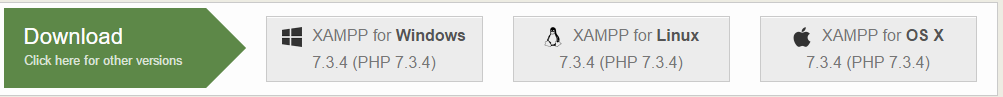
\includegraphics[scale=0.5]{figures/xampp}
\caption{Versi Terbaru XAMPP}
\end{figure}



